% Options for packages loaded elsewhere
\PassOptionsToPackage{unicode}{hyperref}
\PassOptionsToPackage{hyphens}{url}
%
\documentclass[
]{article}
\usepackage{amsmath,amssymb}
\usepackage{lmodern}
\usepackage{iftex}
\ifPDFTeX
  \usepackage[T1]{fontenc}
  \usepackage[utf8]{inputenc}
  \usepackage{textcomp} % provide euro and other symbols
\else % if luatex or xetex
  \usepackage{unicode-math}
  \defaultfontfeatures{Scale=MatchLowercase}
  \defaultfontfeatures[\rmfamily]{Ligatures=TeX,Scale=1}
\fi
% Use upquote if available, for straight quotes in verbatim environments
\IfFileExists{upquote.sty}{\usepackage{upquote}}{}
\IfFileExists{microtype.sty}{% use microtype if available
  \usepackage[]{microtype}
  \UseMicrotypeSet[protrusion]{basicmath} % disable protrusion for tt fonts
}{}
\makeatletter
\@ifundefined{KOMAClassName}{% if non-KOMA class
  \IfFileExists{parskip.sty}{%
    \usepackage{parskip}
  }{% else
    \setlength{\parindent}{0pt}
    \setlength{\parskip}{6pt plus 2pt minus 1pt}}
}{% if KOMA class
  \KOMAoptions{parskip=half}}
\makeatother
\usepackage{xcolor}
\usepackage[margin=1in]{geometry}
\usepackage{graphicx}
\makeatletter
\def\maxwidth{\ifdim\Gin@nat@width>\linewidth\linewidth\else\Gin@nat@width\fi}
\def\maxheight{\ifdim\Gin@nat@height>\textheight\textheight\else\Gin@nat@height\fi}
\makeatother
% Scale images if necessary, so that they will not overflow the page
% margins by default, and it is still possible to overwrite the defaults
% using explicit options in \includegraphics[width, height, ...]{}
\setkeys{Gin}{width=\maxwidth,height=\maxheight,keepaspectratio}
% Set default figure placement to htbp
\makeatletter
\def\fps@figure{htbp}
\makeatother
\setlength{\emergencystretch}{3em} % prevent overfull lines
\providecommand{\tightlist}{%
  \setlength{\itemsep}{0pt}\setlength{\parskip}{0pt}}
\setcounter{secnumdepth}{-\maxdimen} % remove section numbering
\ifLuaTeX
  \usepackage{selnolig}  % disable illegal ligatures
\fi
\IfFileExists{bookmark.sty}{\usepackage{bookmark}}{\usepackage{hyperref}}
\IfFileExists{xurl.sty}{\usepackage{xurl}}{} % add URL line breaks if available
\urlstyle{same} % disable monospaced font for URLs
\hypersetup{
  pdftitle={TEST rmd Knit},
  pdfauthor={Rochelle Rafn},
  hidelinks,
  pdfcreator={LaTeX via pandoc}}

\title{TEST rmd Knit}
\author{Rochelle Rafn}
\date{2022-08-03}

\begin{document}
\maketitle

\hypertarget{year-olds-shopping-at-hm-whats-that-all-about}{%
\section{50 year olds shopping at H\&M? What's that all
about?}\label{year-olds-shopping-at-hm-whats-that-all-about}}

\hypertarget{question}{%
\subsection{Question}\label{question}}

For those who are unfamiliar with H\&M, it's a fast fashion retailer
known for its affordable, youthful and trendy styles. My whole life I
have been into fashion and who knows? Maybe when I'm 50 I will still be
shopping at H\&M or similar stores, like Zara. However, even in my 30s,
if I venture into H\&M I feel noticeably older than everyone else there.
So, why are there twice as many 50 year olds as people my age and where
are they? This lead me to question, does age actually matter for trendy
stores like H\&M that are perceived as `younger'? Are the different
generational age groups actually purchasing different things? Spoiler
alert, they are not. So what does this mean? Who are these 50 year olds
and why are their purchase habits similar to the 20 somethings?

\hypertarget{context}{%
\subsection{Context}\label{context}}

The importance of these questions lies within the realm of demographics
and marketing. Traditionally we believe that location, age, gender all
matter and make a difference. And\ldots{} they do. But, context is
everything. In order to make appropriate and informed decisions it is
important to do proper analysis to make sure we're not assuming
something about someones age or gender that ends up being incorrect. For
instance, is frequent shopper purchasing these things for themselves or
someone else? That is the beauty of data. We can dive in the deep end
and really see what is beneath the surface of human bias.

\hypertarget{summary}{%
\subsection{Summary}\label{summary}}

I started this project with a very different question in mind. However,
after starting at the broadest level questions, my motivation changed. I
chose to begin with the age distribution of all the customers in the
dataset. I really only did this to verify my own assumption that it
would peak somewhere in the mid 20s and then continue to taper off as
age increased. I was definitely surprised to see this somewhat bimodal
distribution with a second peak around 52 years old. I remember
thinking, ``What?? That is so bizarre.'' Twice as many 50 somethings as
30 somethings seemed just\ldots{} wrong.

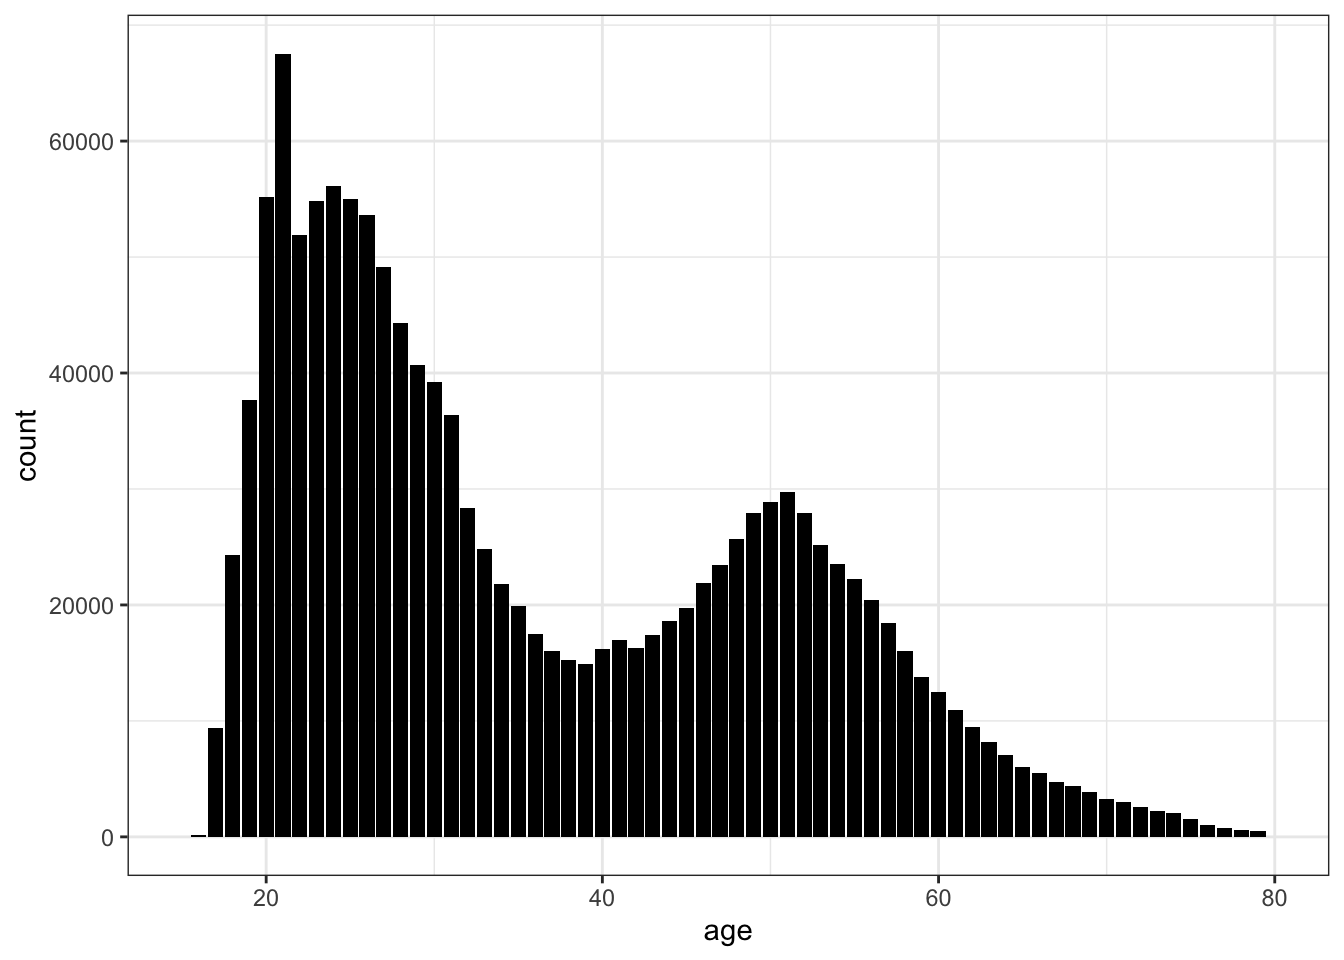
\includegraphics{TEST-rmd-Knit_files/figure-latex/unnamed-chunk-1-1.pdf}

My immediate thought was that it is a group of `young at heart' and
fashion conscious 50 year olds. Then, as I looked a little closer at the
distribution I did the math and realized the peaks moved at very similar
shapes within about 30 years of each other. That logically seems pretty
close to a parent-child age gap. Leading me to question, who are they
actually buying for? My assumption is if the 50 year olds are actually
purchasing for their children, the items would be virtually the same. If
they are actually purchasing for themselves, I should be able to find
some key indicators to predict age.

\hypertarget{data-description}{%
\subsection{Data Description}\label{data-description}}

The data set I'm analyzing comes directly from H\&M spanning 1.3 million
customers (ages 16-99), 53 online markets, 4,850 retail stores and 31
million transactions over 2 years. It came with three relational data
frames with details on Customers, Articles (clothing items) and
Transactions.

\hypertarget{exploratory-data-analysis}{%
\subsection{Exploratory Data Analysis}\label{exploratory-data-analysis}}

Given the question and data that I have, I decided to make age, or age
group, the outcome variable. How can we predict the difference between
the young and mature generations? Or can we at all? To start, I split
the data into the two age groups, ``young'' (\textless=39) and
``mature'' (\textgreater=40). This is where I would start my exploratory
analysis to see what differences I could find.

I began with the most obvious, what are the most popular items in each
age group? Hoping this might show me any key differences. As we can see
here, the top 3 items for both age groups are identical. However, the
fourth item is different. This piqued my interest since that fourth
items seems to indicate an intuitive generational difference. Mature
customers purchased a basic t-shirt, where the young customers purchased
a ``strappy cropped'' top. However, the more I dug, the less significant
this difference became.

\hypertarget{mature-top-items}{%
\subsubsection{Mature Top Items}\label{mature-top-items}}

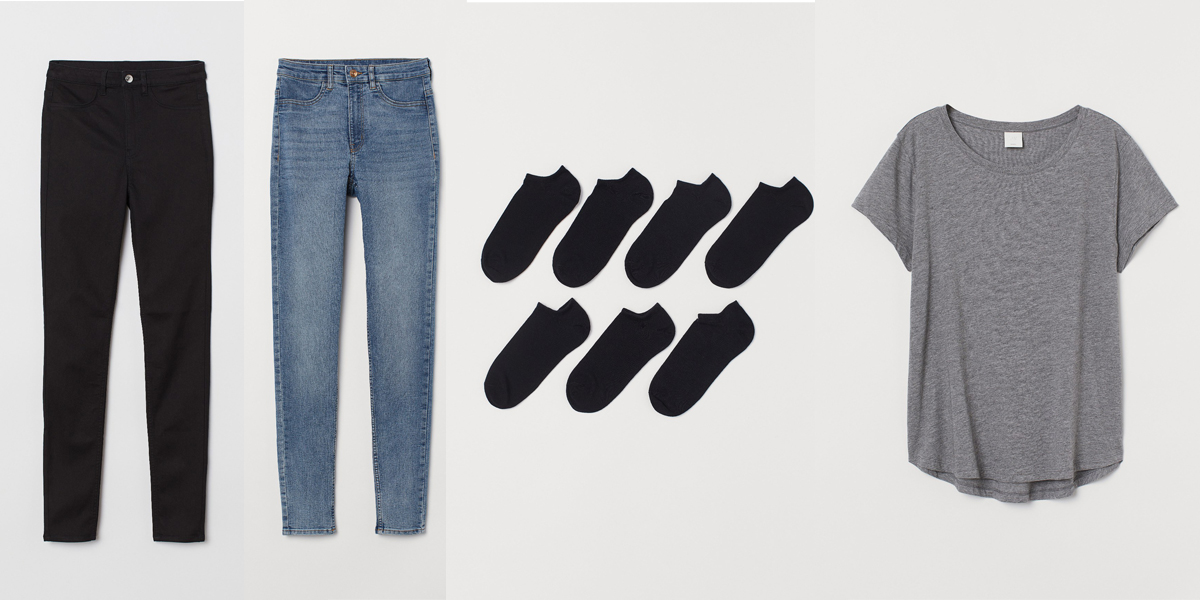
\includegraphics{images/MATURE_top_items.jpg}

\hypertarget{young-top-items}{%
\subsubsection{Young Top Items}\label{young-top-items}}

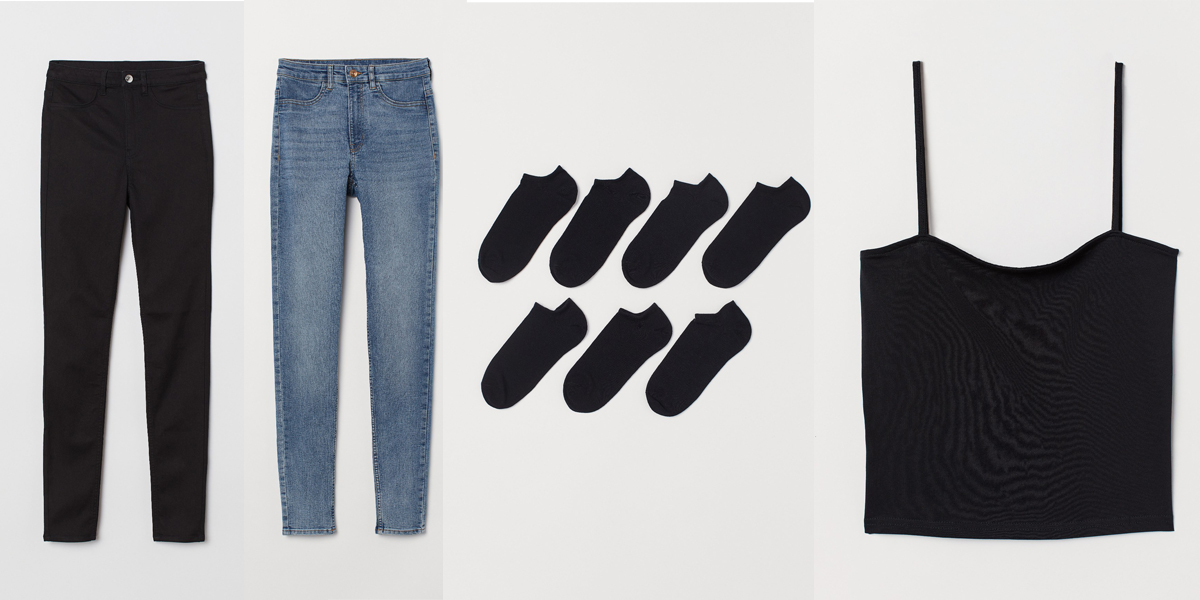
\includegraphics{images/YOUNG_top_items.jpg}

\hypertarget{what-are-the-most-popular-unique-items-in-each-age-group}{%
\subsubsection{What are the most popular unique items in each age
group?}\label{what-are-the-most-popular-unique-items-in-each-age-group}}

From the top items per group, I filtered down even further. I chose to
compare the purchases between the two groups to find unique items. What
items did the young purchase that the mature did not, and vice versa?

\hypertarget{mature-unique-items}{%
\subsubsection{Mature Unique Items}\label{mature-unique-items}}

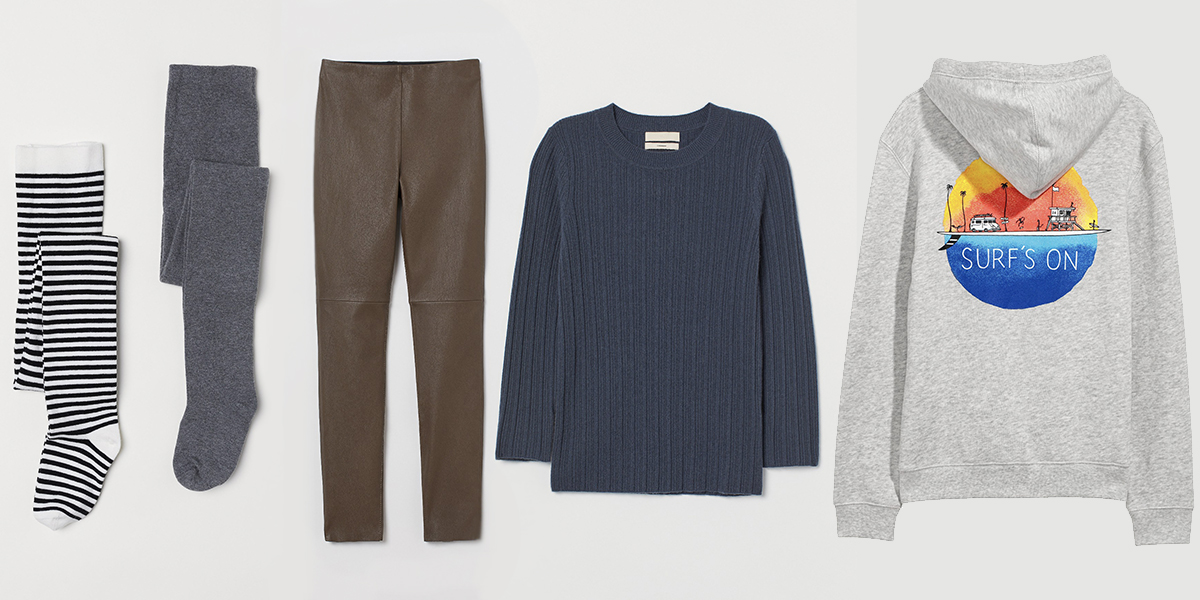
\includegraphics{images/MATURE_unique_items.jpg}

\hypertarget{young-unique-items}{%
\subsubsection{Young Unique Items}\label{young-unique-items}}

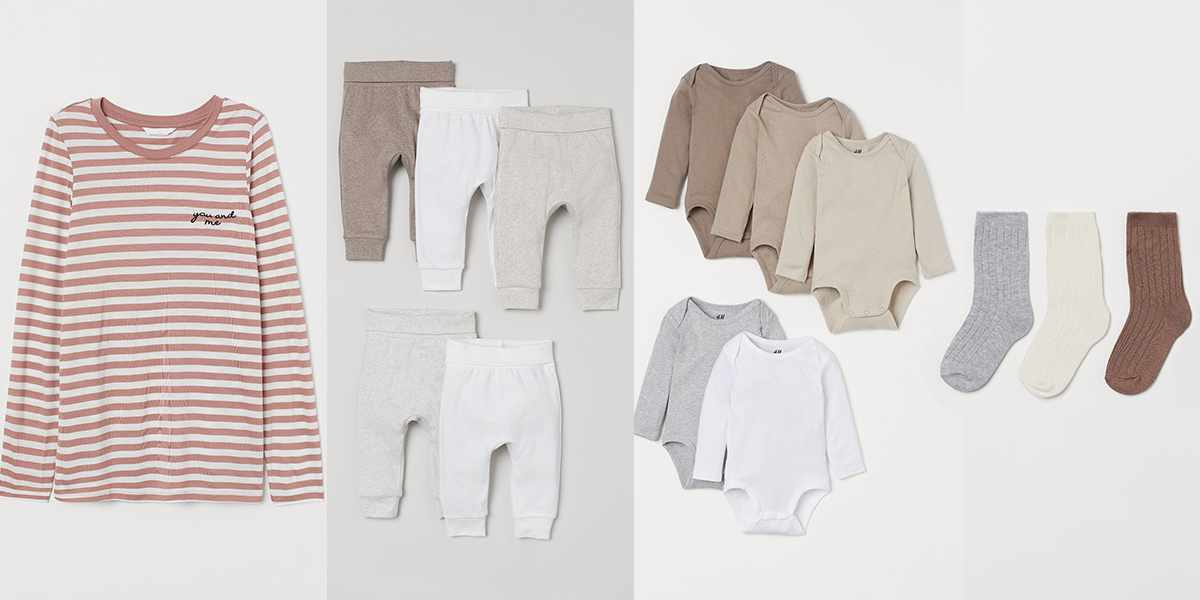
\includegraphics{images/YOUNG_unique_items.jpg}

I started to get a little excited again when I found some interesting
differences between the two groups. In the top items for the young group
there were several baby items. But then the mature group had primarily
items that would be appropriate for an adult child. What if each group
potentially purchases for themselves and their children. For the mature
it would make sense becaue they now have adult children, meaning they
would have no need to purchase baby clothes. However, when I pulled the
counts for these top items each was only purchased at most 86 times out
of more than 21million items purchased. Unfortunately the math here is
not significant enough to consider.

\hypertarget{what-are-the-top-descriptive-words-for-the-unique-items-in-each-age-group}{%
\subsubsection{What are the top descriptive words for the unique items
in each age
group?}\label{what-are-the-top-descriptive-words-for-the-unique-items-in-each-age-group}}

To move forward with the theme of unique items I decided to take those
unique items even deeper by analyzing the descriptive words of these
items. As I had guessed, the unique items really did not hold any
significance due to the small amount. Also, even though the items are
different, there are still many purchases by both groups that have the
same descriptive words despite the specific item differing.

\hypertarget{young-top-word-count}{%
\subsubsection{Young Top Word Count}\label{young-top-word-count}}

\begin{verbatim}
##            word    n
## 1          body 4499
## 2       garment 4488
## 3  babychildren 3628
## 4         sizes 3177
## 5        cotton 2766
## 6         solid 2749
## 7        jersey 2730
## 8          dark 2693
## 9         light 2637
## 10         soft 2613
\end{verbatim}

\hypertarget{mature-top-word-count}{%
\subsubsection{Mature Top Word Count}\label{mature-top-word-count}}

\begin{verbatim}
##            word    n
## 1          body 2295
## 2       garment 2293
## 3  babychildren 1756
## 4      children 1595
## 5          dark 1507
## 6         sizes 1489
## 7         upper 1401
## 8         solid 1345
## 9        jersey 1227
## 10        front 1184
\end{verbatim}

\hypertarget{mature-top-words}{%
\subsubsection{Mature Top Words}\label{mature-top-words}}

\hypertarget{young-top-words}{%
\subsubsection{Young Top Words}\label{young-top-words}}

\hypertarget{what-about-percentage-of-descriptive-words}{%
\subsection{What about percentage of descriptive
words?}\label{what-about-percentage-of-descriptive-words}}

Knowing that there are about twice as many in the young group as the
mature group I thought I would go one step further and check proportion
of the popularity. Still appears that there are no major and obvious
differences.

\begin{verbatim}
##   X graphical_appearance_name pct_difference y_graphic_pct m_graphic_pct
## 1 1                     Solid      3.2125813     57.326729     54.114148
## 2 2          All over pattern      1.1936976     12.085263     13.278961
## 3 3                   Melange      1.0134998      5.609772      6.623272
## 4 4                     Denim      0.8242733      5.918383      6.742657
## 5 5           Other structure      0.6299426      2.498354      1.868411
## 6 6                      Lace      0.5421161      2.048154      1.506038
##   y_graphic_count m_graphic_count
## 1         3459722         1872928
## 2          729357          459594
## 3          338555          229236
## 4          357180          233368
## 5          150778           64667
## 6          123608           52125
\end{verbatim}

\hypertarget{is-there-a-noticeable-difference-in-graphic-appearance-for-each-age-group}{%
\subsubsection{Is there a noticeable difference in graphic appearance
for each age
group?}\label{is-there-a-noticeable-difference-in-graphic-appearance-for-each-age-group}}

When analyzing the number of items with certain graphical appearances it
is almost eerie how mirror like the purchasing habits are. Besides two
variables, they move at extremely similar rates.

\hypertarget{what-is-the-summary-of-price-per-age-group}{%
\subsubsection{What is the summary of price per age
group?}\label{what-is-the-summary-of-price-per-age-group}}

\begin{verbatim}
##      Min.   1st Qu.    Median      Mean   3rd Qu.      Max. 
## 0.0000339 0.0169322 0.0254068 0.0287606 0.0338814 0.5915254
\end{verbatim}

\begin{verbatim}
##      Min.   1st Qu.    Median      Mean   3rd Qu.      Max. 
## 0.0000169 0.0152373 0.0250339 0.0273048 0.0338814 0.5915254
\end{verbatim}

\hypertarget{how-many-items-are-each-group-purchasing-per-transaction}{%
\subsubsection{How many items are each group purchasing per
transaction?}\label{how-many-items-are-each-group-purchasing-per-transaction}}

\begin{verbatim}
##    Min. 1st Qu.  Median    Mean 3rd Qu.    Max. 
##     1.0     3.0     5.0     6.6     8.0   336.0
\end{verbatim}

\begin{verbatim}
##    Min. 1st Qu.  Median    Mean 3rd Qu.    Max. 
##   1.000   3.000   5.000   7.617  10.000 570.000
\end{verbatim}

\end{document}
